\chapter{Design}
\begin{itemize}
    \item This is how I intend to solve the problem! % perhaps here is where I mention stuff like #-stmts and @-stmts?
    \item Builds on the analysis chapter
\end{itemize}

This is when I start comparing Psnodig to the other tools, showing why Psnodig is preferrable etc.

\section{Psnodig}

\subsection{Syntax}

The Psnodig tool in itself is really just a syntax. This syntax includes the standard building blocks like statements, expressions, function declarations, structs etc. However, it also includes two new types of statements, which are specific to our DSL. \hfill \\

\textbf{Hash-Statement}, which can be written like this with BNF: \hfill \\

\textit{HashStmt ::= \# $<$Stmt$>$}. \hfill \\

These statements are read and processed by the interpreter, but ignored during transpiling. They work much like macros do in e.g. the C programming language, but they are declared inside functions, as Psnodig only allows struct- and function declarations to lie in the global scope. They are limited to the line reside in, which makes it easy for the author to decide which lines should be included or ignored when they wish for a different presentation of their code. \hfill \\

\textbf{At-Statement}, which can be written like this with BNF: \hfill \\

\textit{AtStmt ::= @ \{ text \} \{ [$<$Stmt$>$] \}} \hfill \\

These statements consist of two parts, pure text in the first scope, followed by new statements in the second scope. The second part is meant for the interpreter, whilst the first part is meant for the transpilers. This allows the author to abstract over implementation-specific details and/or messy code, which is not crucial for the program's logic. The statement list can also be an empty list, which also makes this a way of letting the author explain things solely with natural language when deemed necessary. \hfill \\

In addition to the syntax, the tool comes with a parser and interpreter for the Gourmet programming language, designed as a proof of concept for this thesis. It also comes with two writers, one presenting the source code with pseudocode, and the other presenting the source code in the form of a flowchart. The main benefit is that we can write our code once in Gourmet, test it, and when we are satisfied, transpile it to pseudocode and/or flowcharts thorugh the command line, rather than having to re-write it manually. \hfill \\

To the best of our knowledge, a tool which combines these methods does not already exist.

\subsection{Interpreter}

\subsection{Gourmet}

\subsection{TBP Writer}

\subsection{IBP Writer}

One of the biggest difficulties with the TikZ library, is that we first have to ``declare'' all of our nodes, before adding edges between them. This means we have to store them somehow, and then later knowing where each edge is coming from and going to. This could be done with a Map. \\

For instance, imagine you have this program:

\begin{lstlisting}
    func Fibonacci(n int) {
        if n <= 2 {
            return 1
        }
        return Fibonacci(n-1) + Fibonacci(n-2)
    }
\end{lstlisting}

This will give us quite a few nodes. I can imagine this:

\begin{itemize}
    \item func Fibonacci(n int)
    \item if n $<=$ 2
    \item return 1
    \item return Fibonacci(n-1) + Fibonacci(n-2)
\end{itemize}

Really we get a node per statement, in addition to the function declaration for good measure. Now, nodes with TikZ are written something like this

\begin{lstlisting}
    \node (name1) [func] {Fibonacci(n)};
    \node (name2) [stmt, below of=name1] {n <= 2};
    ...
\end{lstlisting}

As we can see, each node needs their own unique name, so that they can reference each other later. The square brackets denote necessary metadata, like how the node should look like (declared earlier, here we see func and stmt), their position (for instance, name2 is below name1) etc. Lastly, the curly brackets indicate the text withing the box, displayed on the screen. In listing ? we opted for the function name, and the expression inside the if. \\

Then, after all nodes have been declared, we can start drawing the edges between them, like for instance

\begin{lstlisting}
    \draw [arrow] (name1) -- (name2);
    \draw [arrow] (name2) -- (name3);
    ...
\end{lstlisting}

Thus, we could have a mapping from the function name to the first statement, and thereafter a mapping from that expression to the subsequent expressions. Since we are dealing with an if statement (and followingly an implicit else-statement), a mapping could look something like this

\begin{lstlisting}
    name1 -> name2
    name2 -> name3
    name3 -> name4
    name3 -> name5
\end{lstlisting}

because drawing the edges only really need the labels. The main issue here is that we cannot write the nodes and edges in the same go. \\

However, when working with large control flows with multiple else-branches, we are met with a new dillemma. Simply putting ``a below of$=$c'' and ``b below of$=$c'' will but both a and b on the same spot, and the latter will shadow the former. \\

What we need then is to space them out more evenly, suddenly expanding the metadata to more intricate details like

\begin{lstlisting}
    [stmt, below left of=name3, yshift=-0.5cm, xshift=-1.5cm];
\end{lstlisting}

Additionally, having multiple straight edges from the same source might interfere with each of the edge labels. Thus, we might also have to change the way we draw edges, for instance like this

\begin{lstlisting}
    \draw [arrow] (name3) |- (name5);
\end{lstlisting}

This will curve the edge between name3 and name5, making the flowchart clearer. This is, however, a difficult task to carry out since we never know how programs turn out. Therefore it seems natural to opt for the easiest choice available, and instead, unfortunately, force the authors of tweaking the resulting LaTeX on their own. \\

Another issue is that all control statements have implicit else branches. Take the Fibonacci code above as an example. Technically, the last return statement is the result of an implicit else in the control statement. \\

Now, what is actually interesting here (should be in chapt 3 I know), is that Code2Flow is not always too sure about this stuff either. For instance, this code

\begin{lstlisting}
    Fib() {
        if a { return x }
        else if b { return y }
        else { return z }

        if c { return k }
    }
\end{lstlisting}

actually yields this flowchart

\begin{figure}[ht]
    \centering
    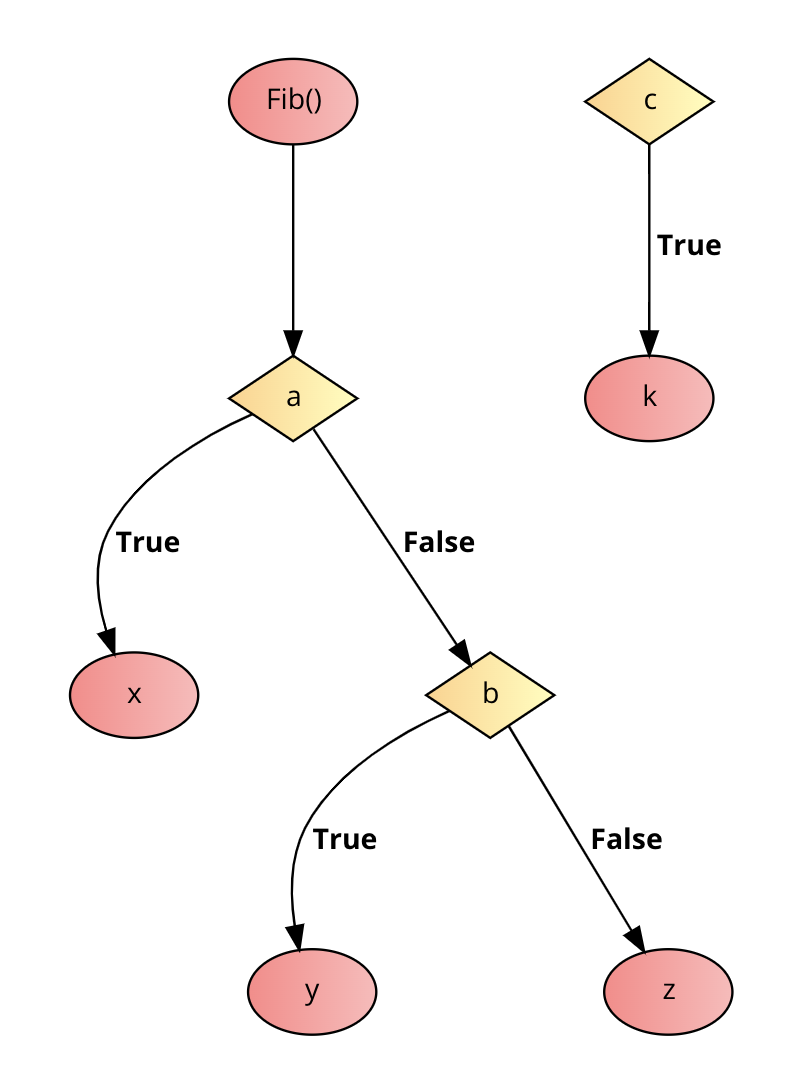
\includegraphics[scale=0.4]{assets/weirdFlowchartC2F.png}
    \caption{IBP from Code2Flow}
    \label{fig:c2f_weird}
\end{figure}

As you can see, the first control sequence is pointed to by the function name, but not the second. This is because all the branches in the first sequence return something (with an explicit else), thus we cannot ever reach the second one. Therefore, it just dangles in the air. \\

However, if we remove the explicit else branch, like so

\begin{lstlisting}
    Fib() {
        if a { return x }
        else if b { return y }

        if c { return k }
    }
\end{lstlisting}

we see that the last control sequence will still act as some sort of else branch

\begin{figure}[ht]
    \centering
    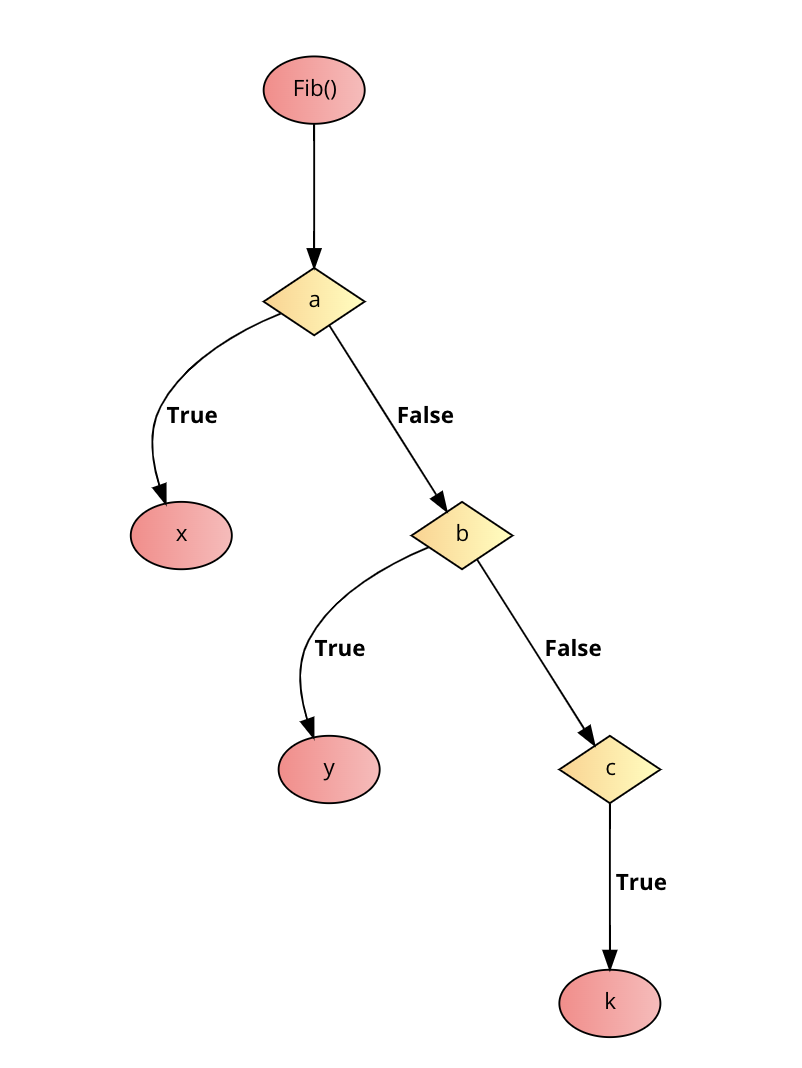
\includegraphics[scale=0.45]{assets/weirdFlochartC2F2.png}
    \caption{More IBP from Code2Flow}
    \label{fig:c2f_weird2}
\end{figure}